% !TeX spellcheck = en_GB

\documentclass{article}

% % % packages % % %
%\usepackage{pdfpages}
\usepackage[titletoc,title]{appendix}
%\usepackage{cite}
%\usepackage{booktabs}
\usepackage{graphicx}
\usepackage{epstopdf}
%\usepackage{caption}
%\usepackage{subcaption}
%\usepackage{dsfont}
%\usepackage{natbib}
%\usepackage{colortbl}
\usepackage{xcolor}
%\usepackage{amsmath}
%\usepackage{amssymb}
%\usepackage{fancyvrb}
\usepackage{listings}
%\usepackage{wrapfig}
%\usepackage{algorithmicx}
%\usepackage{algorithm}
%\usepackage{algpseudocode}
\usepackage{geometry}
\usepackage{hyperref} % always last

% % % custom margins % % %
%\geometry{tmargin=2.2cm, bmargin=2.2cm, lmargin=3cm, rmargin=3cm}

% % % titling % % %
\title{Project Report\\Genetic Algorithms and Evolutionary Computing [H02D1A]}
\author{Jasper Bau, Daan Seynaeve}

\begin{document}

% % % cover % % %
\maketitle
%\newpage

% % % report % % %

\section{Parameter Experiments}

\begin{verbatim}
rondrit16.tsp
--
default settings:
3.5837

Cannot be optimal. Visibile inneffiencies in the tour. Can be optimized by changing only 2 edges. (sometimes)

run 1
Best solution was already there 50 generations ago

run2
not the case


minder generaties (100 default):
50: 3.81, 4.10, 4.01, 3.56, 3.81
(meer crossing edges)
(greater tour length)

25: 3.94, 4.17, 3.57, 4.2, 4.3


minder individuals (50 default):
25: 4.07, 3.55, 3.58, 3.64, 3.07
(less diversity)

meer indivduals:
200: 3.49, 3.45, 3.35, 3.36, 3.41
(consistent result, no crossing edges)

100 individuals, 50 gen:
3.66, 3.67, 3.50, 3.51, 3.54


No elites:
(No convergence, oscillating, random behaviour)
bad results
more generations --> no influence
more individuals --> less extreme oscillation. Average fitness levels out. Seems to be stuck at suboptimal solutions.

More individuals warrants more elite?

High amount of elites -> stuck at specific solutions for a long time. Population converges to a single fitness value.

Enabling loop detection -> much better performance. Faster saturation + convergence.

Prob. for mutation or crossover must be high enough for anything to happen...

If no mutation -> algo can become 'stuck'.

no mutation + low crossover prob -> algo comes to an early stop.

crossover increasingly important for larger problem instances?


\end{verbatim}

\section{Path Representation}

Some operators: \ref{code:cycle_cross} and \ref{code:scx}

\begin{figure}
\centering
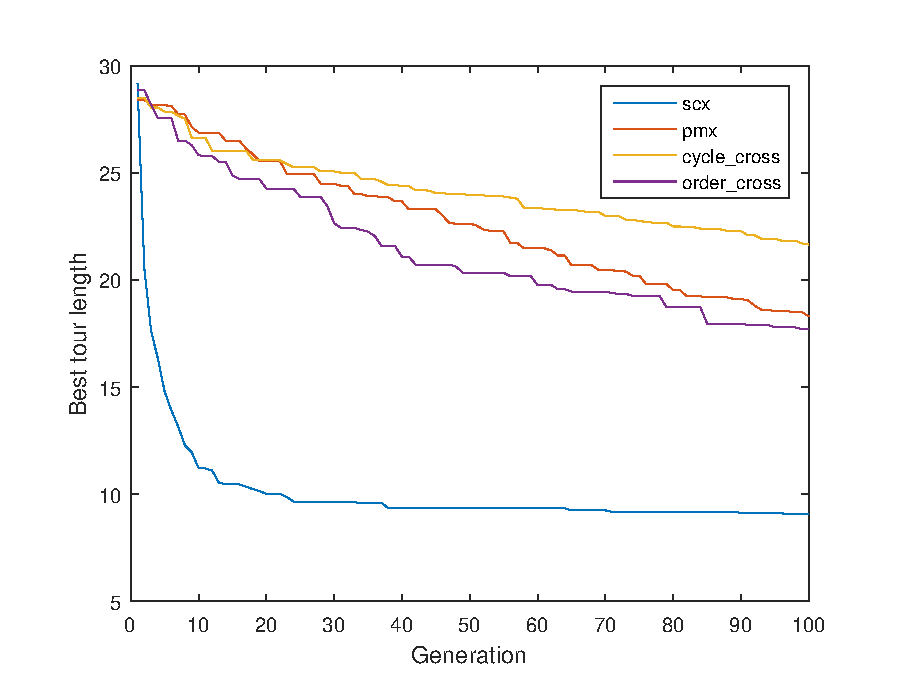
\includegraphics[width=.5\textwidth]{img/rondrit127-pathvs-inv-50-100-20mut-noloop.eps}
\caption{Comparison of path representation crossover operators on the rondrit127 dataset (50 individuals, 95\% crossover, 20\% inversion mutation, no local loop optimization)}
\end{figure}

\section{Optional Task}

\section{Benchmark Performance}

\subsection{rbx711}

\begin{figure}
\centering
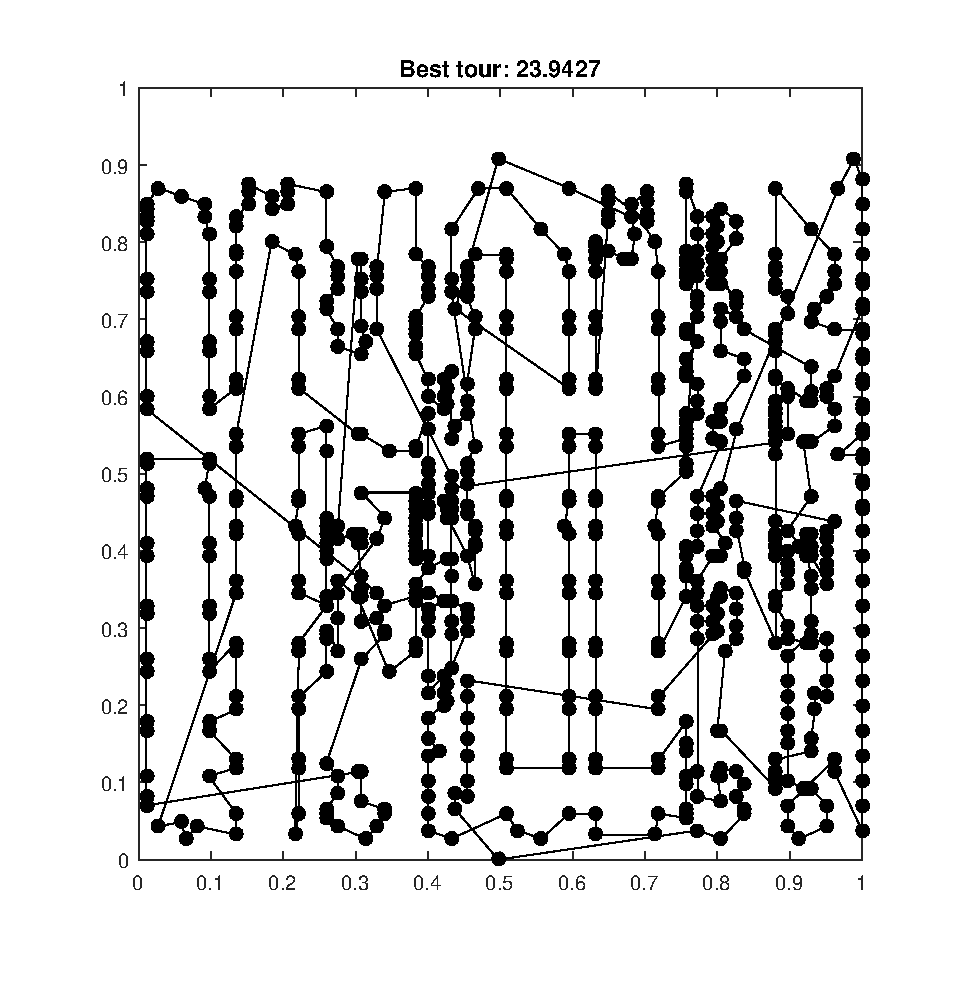
\includegraphics[width=.5\textwidth]{img/rbx711-scx-inv-100-100-35mut-loop.eps}
\caption{rbx711 benchmark: result of 100 generations with a population size of 100 using SCX crossover (95\%) with inversion mutation (35\%).}
\end{figure}


% % % appendices % % %
\newpage
\newgeometry{tmargin=2cm, bmargin=2cm, lmargin=2cm, rmargin=2cm}
\lstset{
	language=Matlab,
	basicstyle=\footnotesize,
	commentstyle=\color{gray},
	numbers=left,
	numberstyle={\tiny \color{black}},
	numbersep=9pt
}
\begin{appendices}
\section{Code}
\subsection{scx.m}\label{code:scx}
	\lstinputlisting{../ga/template/crossovers/scx.m}
\subsection{pmx.m}\label{code:pmx}
	\lstinputlisting{../ga/template/crossovers/pmx.m}
\subsection{cycle\_cross.m}\label{code:cycle_cross}
	\lstinputlisting{../ga/template/crossovers/cycle_cross.m}
\subsection{order\_cross.m}\label{code:order_cross}
	\lstinputlisting{../ga/template/crossovers/order_cross.m}
\subsection{run\_ga\_adapted.m}\label{code:run_ga}
	\lstinputlisting{../ga/template/run_ga_adapted.m}
\end{appendices}
\restoregeometry

\end{document}
